Dynamic parallelism is a "relative" new feature in the \cuda{} programming model.
It was added in \cuda{} 5.0 and it allows kernels to launch other kernels i.e threads can launch more threads.
An example of nested parallelism can be seen in \autoref{fig:nested-kernel} (The letters symbolizes kernels inside a \cuda{} stream).
Kernels A,B and C are launched by the host (Parent)
When kernel B executes, it launches kernels D, E and F (Children) and when kernel E executes, it launches G,H and I (Grand children).
\begin{figure}[ht]
	\centering
	\fbox{
		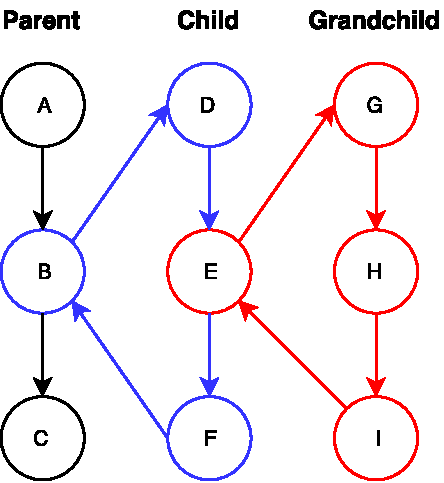
\includegraphics[width=0.3\textwidth]{figs/programming-model/recursive-kernel.pdf}
	}
	\caption{Nested kernel call}
	\label{fig:nested-kernel}
\end{figure}
The feature was added to express nested and recursive parallelism more easily, as this type of parallelism arises naturally in many applications.
An example is quick sort which is a "divide and conquer" algorithm which is well suited for recursion.
The idea is that an element is picked (called a pivot point), and all elements less that this point is reordered to come before the pivot point, and all points larger to come after.
This is performed recursively until all elements have been sorted.
An example can be seen in \autoref{fig:recursion-quicksort}
\begin{figure}[ht]
	\centering
	\fbox{
		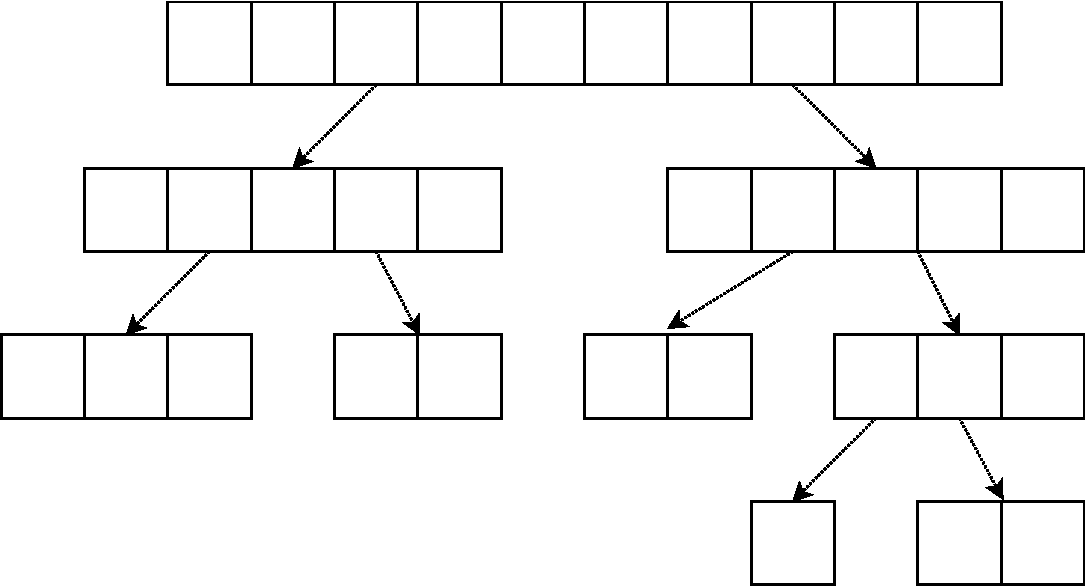
\includegraphics[width=0.4\textwidth]{figs/programming-model/recursion-quicksort.pdf}
	}
	\caption{Recursion and quicksort}
	\label{fig:recursion-quicksort}
\end{figure}

Launching kernels from within other kernels can be beneficial in some applications, but there are also things to watch out for when using this technique in \cuda{}.
Shared memory cannot be passed to a child kernel, so there is a performance penalty in having to copy data to global memory.
One should also be aware that every thread is executing the same program/kernel, which means that every thread will launch child kernels.